\chapter{Métodos de Construção e Uso de Datasets de EEG e ET}


Lu et al. (2015) faz uso de dados de EEG e ET para classificação de emoções nas três 
valências emocionais eleitas no estudo de Zheng et al. (2014). Em contraste com o volume de 
informações coletadas no estudo de Zheng et al., Lu et al. coletam uma 
maior quantidade de dados de rastreamento ocular – 
extraindo 16 métricas de ET, enquanto o estudo de Zheng foca em apenas 
métricas principais da dilatação ocular. 
Os resultados da acurácia do algoritmo aplicado aos diferentes métodos de fusão 
de dados multimodais estão resumidos na imagem 5.2, 
ficando evidente que, independente do método utilizado para fusão das modalidades de EEG e ET, 
as melhores acurácias foram encontradas para base de dados de mais de uma fonte de informação 
fisiológica. 


\begin{figure}
      \centering
      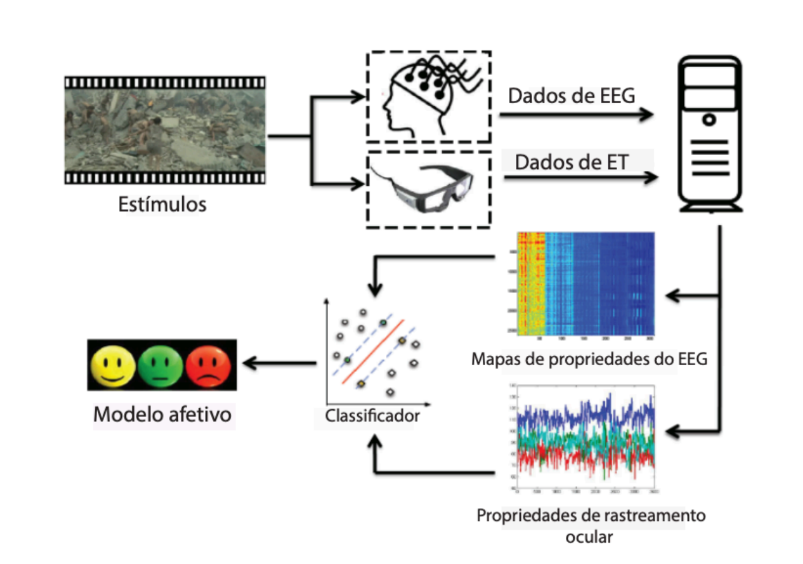
\includegraphics[width=150mm]{estimulo_e_coleta.png}
      \caption{Design de Experimento para Coleta de EEG e ET. Fonte: Zheng et al. (2014)}
\end{figure}


\begin{figure}
      \centering
      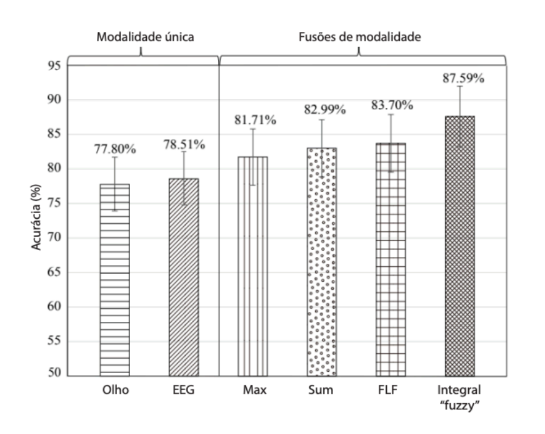
\includegraphics[width=100mm]{lu.png}
      \caption{Acurácia por Método de Fusão de Modalidade e Modalidade Única em Algoritmo Supervisionado. Fonte: Lu et. al. (2015)}
\end{figure}

No trabalho de Thapaliya et al. (2019) dados de EEG e ET foram aplicados em algoritmos de máquina, 
com o objetivo de estudar uma melhora no método de diagnóstico de crianças com autismo através de 
diferentes formas de pré-processamento (exemplo de processamento do estudo na figura 5.3). 
Os dados de EEG tiveram suas métricas estatísticas coletadas para a construção de um vetor de características 
(incluindo desvio padrão e média por janela de tempo dos dados de EEG filtrados), assim como a entropia calculada 
por janela temporal. Para os dados de ET, os tempos de fixação foram coletados, em conjunto com o resultado de testes cognitivos. 
Em seu estudo, diferentes métodos de construção de vetores de características foram analisados, 
tanto para os dados unimodais quanto para a junção de EEG e ET. 


\begin{figure}[h]
      \centering
      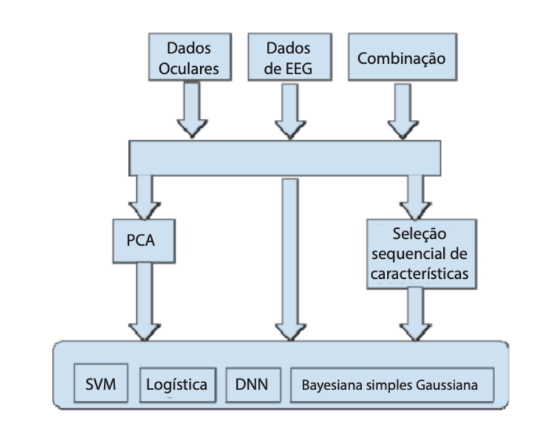
\includegraphics[width=100mm]{thapalya.png}
      \caption{União de dados de EEG e ET. Fonte: Thapaliya et al. (2019)}
\end{figure}

Através das acurácias apresentadas para os diferentes métodos de processamento, 
é possível observar que determinados algoritmos aumentaram sua acurácia a
 depender do modo no qual o vetor de características foi construído. 
 Por exemplo, enquanto o algoritmo Support Vector Machine (SVM) atingiu \textbf{71\%} de acurácia 
 com o vetor que incluiu Entropia para as janelas de EEG e PCA, a regressão logística com maior acurácia 
 foi atingida com o dataset de desvio padrão de EEG e dados de rastreamento ocular sem a aplicação de PCA 
 (Thapaliya et al., 2019). 

Lim e Chia (2015), estudaram a correlação de ondas EEG detectadas em um equipamento de eletrodo único e 
estresse cognitivo induzido pelo teste de Stroop. A análise foi feita com base na aplicação de três algoritmos: 
\textit{Artificial Neural Network}, \textit{k-Nearest Neighboor} (KNN) e \textit{Linear Discriminant Analysis} (LDA), 
dos dados de EEG transformados pela aplicação da Transformação Cosseno Discreta (\textit{Discrete Cosine Transform} – DCT). 
O KNN com o DCT conseguiu classificar melhor o estado de estresse do participante.

\chapter{Equipamentos Comerciais na Pesquisa}

O uso do MindWave Mobile II foi recentemente empregado para o 
controle de cadeira de rodas (Abuzaher e Al-Azzeh, 2021; Permana et al., 2019), 
controle de mão robótica e robô móvel (Purnamasari et al., 2019; Rusanu et al., 2019; Rușanu et al., 2021) 
e predição de personalidade (Bhardwaj et al., 2021). 

Outro estudo com uso de eletrodo único como fonte de dados eletrofisiológicos foi o trabalho de Quesada-Tabares et al. (2017), 
onde foi demonstrado que o uso de EEG comercial e com eletrodo único também possui um importante poder classificatório 
quando aplicado em algoritmos. Em seu estudo, sete participantes observaram imagens selecionadas do 
\textit{International Affective Picture System} (IAPS) pertencentes a três grupos com diferentes valores de 
valência e excitabilidade. O teste de Análise de Variância aplicado indicou 
uma diferença estatisticamente significante entre os sets de imagens.
 Um segundo teste foi conduzido pela aplicação de um algoritmo de classificação no estilo árvore de decisão,
  chegando a uma acurácia média entre os sete participantes de \textbf{80.71\%}.

Bos (2021) também explora o uso do Mindwave no contexto escolar para medir a atenção dos alunos. Em seu estudo, 
o nível de atenção com alunos assistindo a um vídeo educacional sem e outro com interações (fazendo pergunta aos alunos)
 é explorado e a distribuição percentual das diferentes bandas de frequência são comparadas entre os grupos. Foi 
 observado uma relativa diminuição banda de frequência de onda beta para o grupo que não assistiu ao vídeo interativo, 
 o que foi relacionado a um processamento cognitivo reduzido e menor atenção.


%Bhardwaj et al. (2021) analisou o uso dos dados coletados com o Mindwave para classificar sete traços de personalidade 
%com o algoritmo \textit{deep long short term memory} (DeepLSTM) e tratando os dados com transformada de Fourier Rápida. 
%A pesquisa contou com 50 participantes (25 mulheres e 25 homens), com idades entre 18 e 46 anos, e durou cinco dias.
%Os dados foram coletados enquanto os participantes assistiam vídeos relacionados a traços de personalidade. 
% Os traços foram separados de acordo com os tipos de personalidade definidos no \textit{Myers-Briggs Type Indicator}, 
% e ao final de cada vídeo, o participante deveria dizer se concordava, 
% discordava ou era neutro aos questionários de personalidade sobre o traço proeminente no estímulo. 
% O questionário de cada participante foi utilizado para determinar o traço de personalidade, 
% que serviria para então classificar os dados em três possíveis outputs: 
% (a) participante tem traço de personalidade apresentado no vídeo, (b) participante não tem traço apresentado de forma significativa 
% e (c) participante tem traço oposto ao apresentado no vídeo.
 
% [FALTOU CONCLUSÃO AQUI]



\section{Considerações Finais}
Datasets multimodais tendem a performar melhor em algoritmos classificatórios que datasets unimodais. 
A forma de processamento dos dados também pode ter impactos na performance classificatórias dos algoritmos. 
Equipamentos comerciais já foram previamente utilizados em estudos de algoritmos classificatórios. 
É esperado que um método de tratamento eficiente reflita em uma maior acurácia dos algoritmos treinados no dataset. 

